\documentclass[tikz,border=8pt]{standalone}
\usepackage{amsmath}
\usepackage{amssymb}
\usetikzlibrary{arrows.meta,calc,positioning}

\definecolor{ridgeblue}{HTML}{2F6F9F}
\definecolor{ridgegold}{HTML}{B7791F}
\definecolor{ridgegreen}{HTML}{4F7C5B}
\definecolor{textgray}{HTML}{2F3437}
\definecolor{linegray}{HTML}{AEB7BC}

\begin{document}
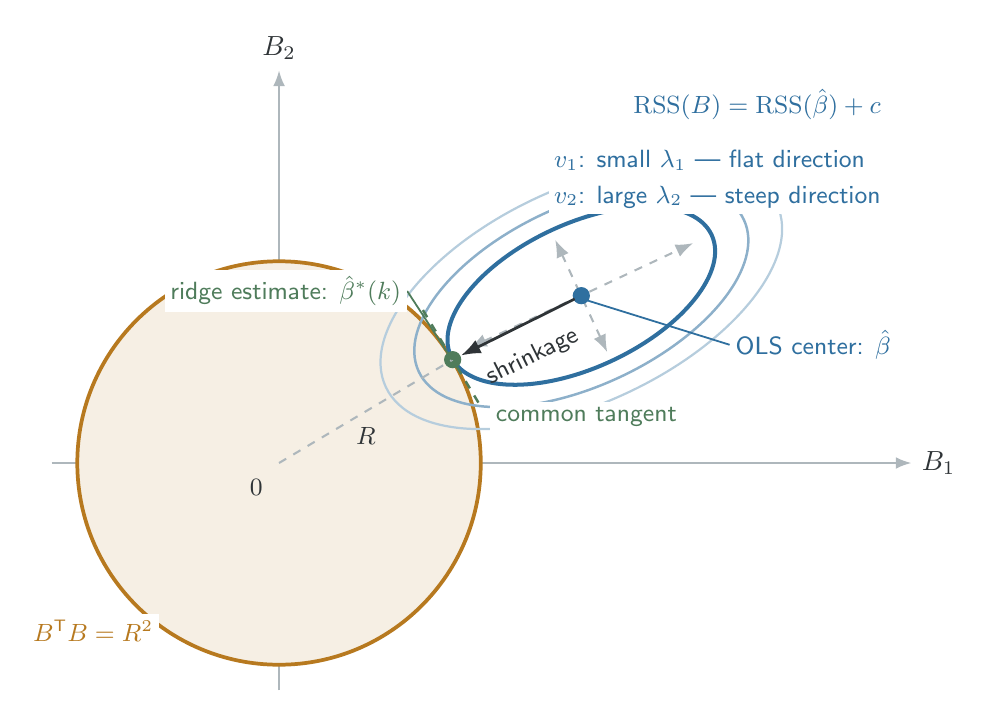
\begin{tikzpicture}[
  x=1.05cm,
  y=1.05cm,
  font=\sffamily,
  >=Latex,
  axis/.style={-{Latex[length=2mm]}, draw=linegray, line width=0.8pt},
  guide/.style={draw=linegray, dashed, line width=0.75pt},
  movement/.style={-{Latex[length=2.5mm]}, draw=textgray, line width=1pt},
  point/.style={circle, inner sep=2.2pt},
  label/.style={font=\sffamily\small, text=textgray},
  mathlabel/.style={font=\sffamily\small, text=textgray, fill=white, inner sep=2pt}
]

% Coefficient-space coordinates.  The chosen ellipse and circle satisfy the
% ridge KKT tangency condition at beta_ridge.
\coordinate (origin) at (0,0);
\coordinate (ols) at (3.656,2.024);
\coordinate (ridge) at (2.100,1.250);

% Axes in the two-dimensional coefficient plane.
\draw[axis] (-2.75,0) -- (7.65,0) node[right, text=textgray] {$B_1$};
\draw[axis] (0,-2.75) -- (0,4.75) node[above, text=textgray] {$B_2$};

% The feasible coefficient-length sphere (a circle in two dimensions).
\fill[ridgegold!12] (origin) circle[radius=2.44];
\draw[draw=ridgegold, line width=1.35pt] (origin) circle[radius=2.44];
\node[mathlabel, text=ridgegold, anchor=north east] at (-1.45,-1.82)
  {$B^{\mathsf T}B=R^2$};

% Nested residual-sum-of-squares contours centered at the OLS estimate.
% The long principal direction corresponds to the smaller eigenvalue.
\begin{scope}[rotate around={25:(ols)}]
  \draw[draw=ridgeblue!35, line width=0.8pt]
    (ols) ellipse[x radius=2.61, y radius=1.30];
  \draw[draw=ridgeblue!55, line width=0.9pt]
    (ols) ellipse[x radius=2.17, y radius=1.09];
  \draw[draw=ridgeblue, line width=1.45pt]
    (ols) ellipse[x radius=1.739, y radius=0.870];
\end{scope}

\node[mathlabel, text=ridgeblue, anchor=east] at (7.35,4.34)
  {$\operatorname{RSS}(B)=\operatorname{RSS}(\hat\beta)+c$};

% Principal axes of the RSS ellipses.
\draw[guide, <->] (2.30,1.39) -- (5.01,2.66);
\draw[guide, <->] (3.97,1.34) -- (3.34,2.70);
\node[mathlabel, text=ridgeblue, anchor=north east, align=left]
  at (7.35,3.86)
  {$v_1$: small $\lambda_1$ --- flat direction\\[2pt]
   $v_2$: large $\lambda_2$ --- steep direction};

% OLS and ridge estimates.
\node[point, fill=ridgeblue] at (ols) {};
\draw[draw=ridgeblue, line width=0.65pt] ($(ols)+(0.08,-0.06)$) -- (5.45,1.43);
\node[mathlabel, text=ridgeblue, anchor=west] at (5.45,1.43)
  {OLS center: $\hat\beta$};

\node[point, fill=ridgegreen] at (ridge) {};
\draw[draw=ridgegreen, line width=0.65pt] (1.55,2.08) -- ($(ridge)+(-0.06,0.08)$);
\node[mathlabel, text=ridgegreen, anchor=east] at (1.55,2.08)
  {ridge estimate: $\hat\beta^{*}(k)$};

% Shrinkage path and the radius normal to the tangent point.
\draw[movement] ($(ols)+(-0.08,-0.04)$) -- ($(ridge)+(0.10,0.05)$)
  node[midway, below=4pt, sloped, label] {shrinkage};
\draw[guide] (origin) -- (ridge) node[midway, below=2pt, label] {$R$};

% Common tangent at the constrained optimum.
\draw[draw=ridgegreen, dashed, line width=0.9pt]
  (1.74,1.85) -- (2.46,0.65);
\node[mathlabel, text=ridgegreen, anchor=west] at (2.55,0.56)
  {common tangent};

\node[label, anchor=north east] at (-0.08,-0.08) {$0$};
\end{tikzpicture}
\end{document}
